\subsection{Применение системы компьютерного зрения в антропометрии для фитнеса (E-Fitness)}
Программа <<E-Fitness>> предназначена для фитнеса.
При запуске программы появляется главное окно формы \ref{img38}

\begin{itemize}
\item <<Measure Me>> В рабочей области отображается видеопоследовательность, область обнаружения объектов и извлечение антропометрических признаков;
\item <<Credit>> Контакты с командой разработчиков;
\item <<Exit>> Позволяет осуществить выход из программы.
\end{itemize}

\begin{figure}[ht!]
\centering
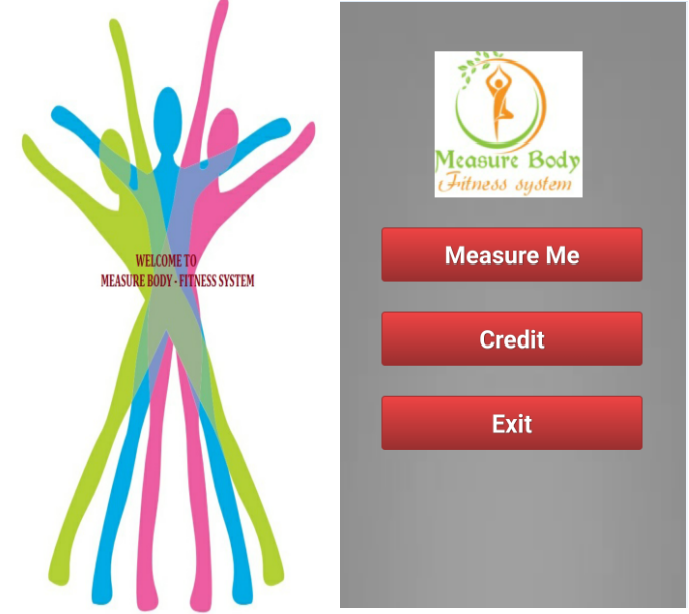
\includegraphics [scale=0.5] {images/h38.png}
\begin{center}
%\captionsetup{justification=justified, labelsep=period}
\caption{Основный интерфейс приложения E-Fitness} \label{img38}
\end{center}
\end{figure}

\textbf{Основные функции приложения E-Fitness}\ref{img39}

\begin{itemize}
	\item Позволять пользователям добавлять информацию;
	\item Показать 3D-модель на основе антропометрических признаков и классификации данных \ref{img40};
	\item Анализ антропометрических признаков на основе стандартов Fitness \ref{img41}.
\end{itemize}

\begin{figure}[ht!]
\centering
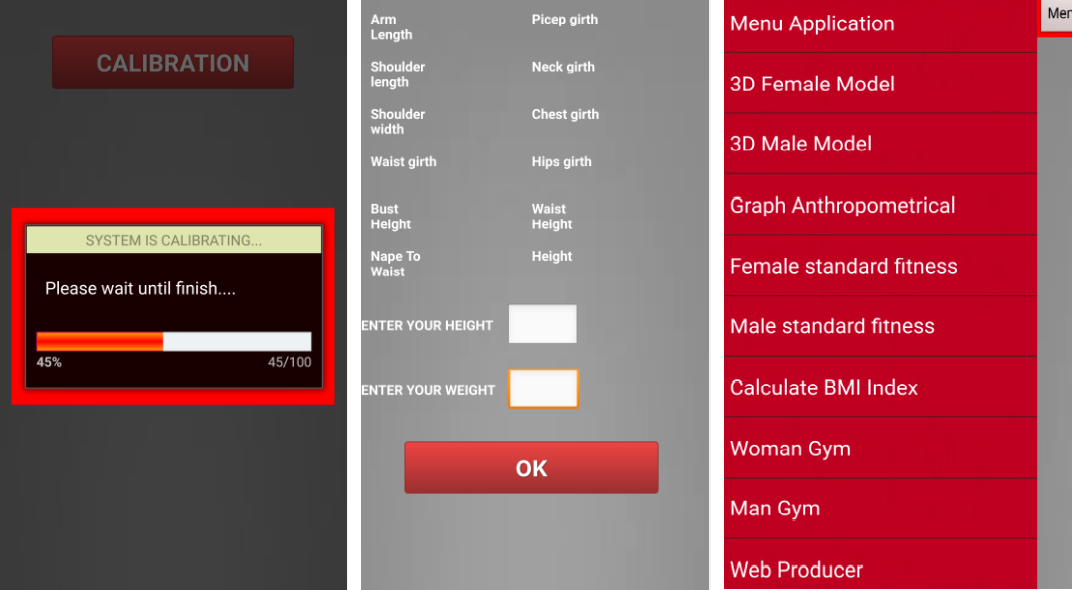
\includegraphics [scale=0.5] {images/h39.png}
\begin{center}
%\captionsetup{justification=justified, labelsep=period}
\caption{Интерфейс работы программы } \label{img39}
\end{center}
\end{figure}

\begin{figure}[ht!]
\centering
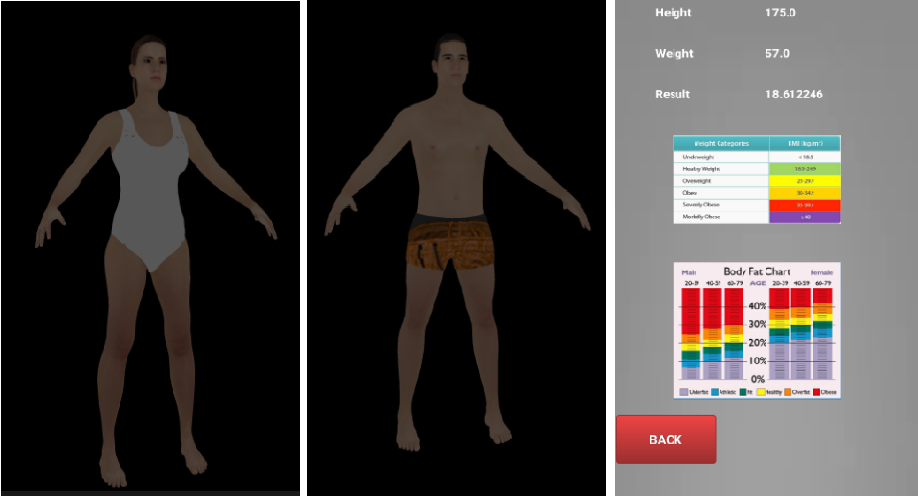
\includegraphics [scale=0.5] {images/h40.png}
\begin{center}
%\captionsetup{justification=justified, labelsep=period}
\caption{Результат 3D-моделей} \label{img40}
\end{center}
\end{figure}
В (рис.\ref{img41}) описывает анализ антропометрических признаков по фитнес-стандартам. Где красная линия - реальные размеры, зеленная линия - размеры по фитнес-стандартам. Приложение позволяет пользователям сравнить свои параметры с размерами по фитнес-стандартам.  
\begin{figure}[ht!]
\centering
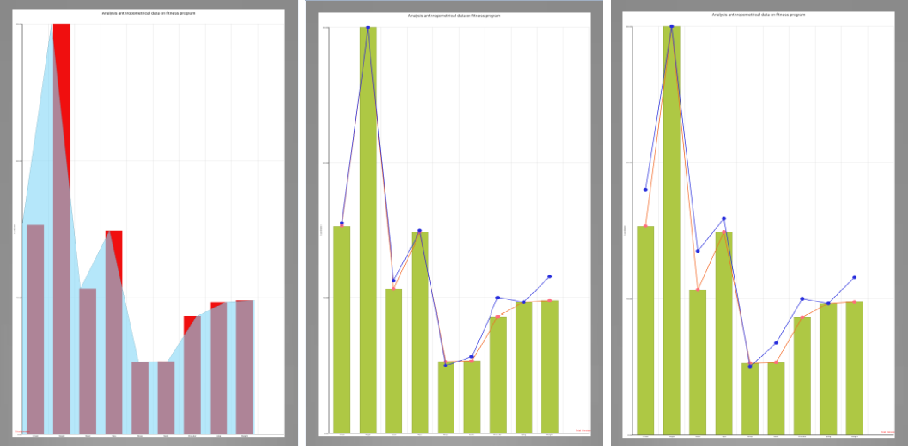
\includegraphics [scale=0.5] {images/h41.png}
\begin{center}
%\captionsetup{justification=justified, labelsep=period}
\caption{Результат анализа антропометрических признаков на основе стандартам Fitness} \label{img41}
\end{center}
\end{figure}